\documentclass[titlepage]{article}
\usepackage{array}
\usepackage{enumerate}
\usepackage{graphicx}
\usepackage{listings}

\begin{document}

\author{Stevan Stanisic and Santana Mach}
\title{COMP 8505 - Final Project \\ Rootkit \\ Design Documents}
\date{Nov 06, 2011}
\maketitle{}

\tableofcontents
\pagebreak

\section{Introduction}

Need an intro...

\section{Program Functionality}

\begin{lstlisting}
Pseudo-code for Client Program
{
  Main Function
  {
    Parse arguments;
    Read config file;

    Pass address into backdoor_client();
  }

  backdoor_client Function
  {
    Verify address and port;

    Setup listening_thread();

    While read stdin
    {
      if exfil switch is set
        set exfil path to send;

      Prepare raw socket;
    }
  }

  listen_thread Function
  {
    Prepare listening socket;

    While socket is open
    {
      Receive packet;
      Decrypt payload;
      Print decrypted payload;
    }
  }
}
\end{lstlisting}

\clearpage

\begin{lstlisting}
Pseudo-code for Server Program
{
  Main Function
  {
    Parse arguments;
    Read config file;

    Mask the process name;

    Pass filter into pcap_init();

    Execute srv_listen();
  }

  pcap_init Function
  {
    Open pcap packet capture;
    Build packet filter;
    Set packet filer;
  }

  srv_listen Function
  {
    Forever Loop
    {
      Process packet and pass into pkt_handler;
    }
  }

  pkt_handler Function
  {
    Locate payload portion of packet;

    Authenticate backdoor header key;

    Return if authentication fails;

    Decrypt payload with DES;

    Verify decrypted contents;

    Extract command from contents;

    Grab return address;

    Pass command and address into execute();
  }

  execute Function
  {
    Run command and grab standard out;

    Prepare raw socket for duplex;

    While content in stdout
    {
      Switch with covert mode;
      Encrypt content with DES;
      Send encrypted content to client;
    }   
  }

  covert_udplen Function
  {
    
  }

  covert_ntp Function
  {
    
  }

  covert_icmp Function
  {
    
  }

  exfil Function
  {

  }
}
\end{lstlisting}

\clearpage

\section{Communication Details}

\subsection{State Machine}

\begin{figure}[htb]                                                                       
  \begin{center}
    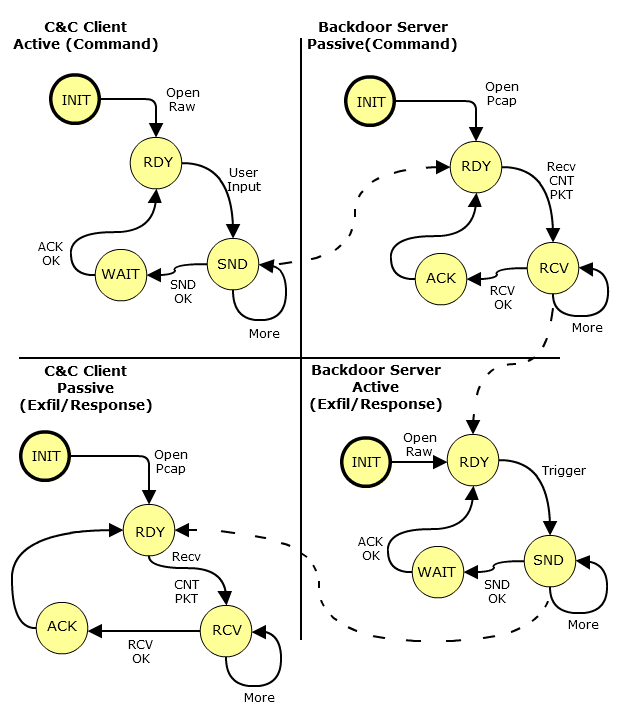
\includegraphics[width=0.9\textwidth]{imgs/std.png}
  \end{center}
  \caption{Program State Transition Diagram}
  \label{fig:std}
\end{figure}

\begin{figure}[htb]                                                                       
  \begin{center}
    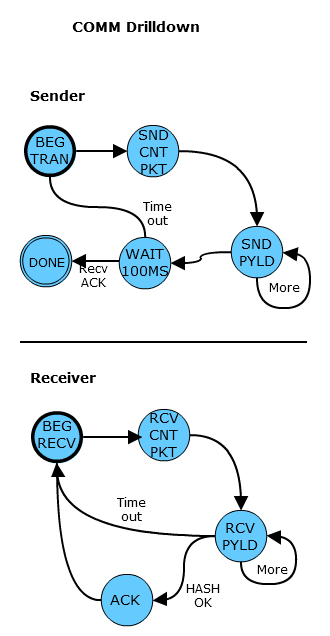
\includegraphics[width=0.5\textwidth]{imgs/comm.png}
  \end{center}
  \caption{Transmission State Transition Diagram}
  \label{fig:comm}
\end{figure}

\begin{lstlisting}
Pseudo-code for State Machine
\{
	Pseudo code goes here

	...
\}
\end{lstlisting}

\clearpage

\subsection{Covert Channel}

\begin{figure}[htb]                                                                       
  \begin{center}
    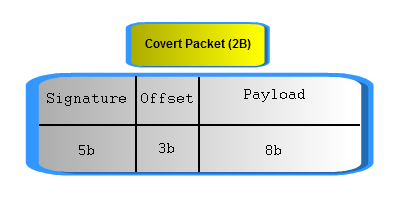
\includegraphics[width=0.9\textwidth]{imgs/packet.png}
  \end{center}
  \caption{Packet Data Diagram}
  \label{fig:packet}
\end{figure}

\begin{figure}[htb]                                                                       
  \begin{center}
    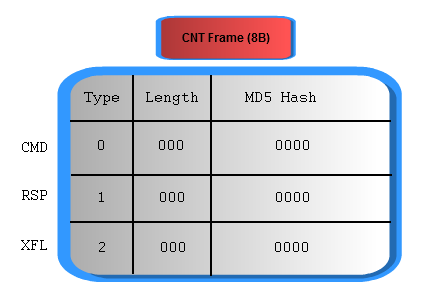
\includegraphics[width=0.9\textwidth]{imgs/frame.png}
  \end{center}
  \caption{Control Frame Diagram}
  \label{fig:frame}
\end{figure}

\begin{figure}[htb]                                                                       
  \begin{center}
    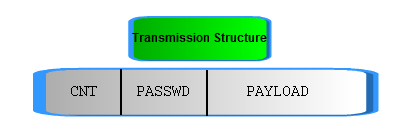
\includegraphics[width=0.9\textwidth]{imgs/transmission.png}
  \end{center}
  \caption{Overall Transmission Diagram}
  \label{fig:transmission}
\end{figure}

\clearpage

\section{Conclusion}

\end{document}
